\chapter{Improvement techniques}\label{cap:ImprovementTechniques}

This chapter documents the implementation of the following techniques used to improve the playing strength of the chess engine:

\begin{itemize}[itemsep=2pt]
    \item Transposition tables with Zobrist hashing.
    \item Move generator with magic bitboards and PEXT instructions.
    \item Evaluation with king safety and piece mobility parameters.
    \item Multithread search.
    \item Search with late move reductions.
\end{itemize}

\section{Transposition table}\label{sec:tt}

\noindent As discused in the previous chapter (see~\cref{sec:iterativeDeepening}), the basic implementation of the chess engine generates a large amount of redundant calculations due to the iterative deepening approach and also the concept of transpositions: situations in which the same board position is reached through different sequences of moves in the game tree.
\noindent~\cref{fig:transposition_example} illustrates a position that can arise through multiple move orders. Where the white king could go to the g3 square from multiple paths.

\begin{figure}
    \centering
    \newchessgame
    \chessboard[
        showmover=false,
        setfen=8/2k5/3p4/p2P1p2/P2P1P2/8/8/2K5 w - - 0 1,
        pgfstyle=straightmove, color=blue,
        markmoves={c1-e3,e3-g3,c1-g1,g1-g3},
        arrow=to
    ]
    \caption{Lasker-Reichhelm Position, transposition example.}\label{fig:transposition_example}
\end{figure}

\vspace{1em}

\noindent Taking advantage of dynamic programming, we create a look-up table of chess positions and its evaluation. So if we encounter the same position again, the evaluation is already precalculated. However, we ask ourselves the following question: how much space does the look-up table take up if there are an astronomical amount of chess positions? What we can do is assign a hash to each position and make the table index the last bits of the hash. The larger the table, the less likely access collisions will be. We also want a hash that is fast to calculate and has collision-reducing properties~\cite{TranspositionTable}.


\vspace{1em}

\noindent \parbox{\textwidth}{The complete implementation can be found in\\\texttt{include\textbackslash{}utilities\textbackslash{}transposition\_table.hpp}.}

\newpage

\subsection*{Zobrist hashing}

Zobrist Hashing is a technique to transform a board position of arbitrary size into a number of a set length, with an equal distribution over all possible numbers invented by Albert Zobrist~\cite{ZobristHashing}.

\vspace{1em}

\noindent To generate a 64-bit hash for a position, the following steps are followed:

\begin{enumerate}
  \item Pseudorandom 64-bit numbers are generated for various features of a position:
  \begin{enumerate}
    \item One number for each piece type on each square (12 pieces x 64 squares).
    \item One number to indicate the side to move is black.
    \item Four numbers to represent castling rights (kingside and queenside for both white and black).
    \item Eight numbers to represent the file of an available \textit{en passant} square.
  \end{enumerate}
  \item The final hash is computed by XOR-ing together all the random numbers corresponding to the features present in the current position.
\end{enumerate}

\noindent These random values ensure that even slightly different positions produce very different hash values. This greatly reduces the chance of collisions.

\vspace{1em}

\noindent The XOR operation is used not only because it is computationally inexpensive, but also because it is reversible. This means that when a move is made or undone, we can update the hash incrementally by applying XOR only to the affected squares, without needing to recompute the entire hash.

\vspace{1em}

\noindent The position shown in~\cref{fig:zobristExamplePosition} illustrates an example of how the Zobrist hash is computed.  
The hash value is calculated by XORing the random values associated with each element of the position.

\vspace{1em}

\noindent Since the side to move is white, we do not XOR the value associated with black to move. The resulting hash is computed as follows:

\[
111 \oplus 69 \oplus 909 \oplus 10 \oplus 67 \oplus 12 \oplus 555 \oplus 3 = 458
\]

\noindent Where $\oplus$ denotes $XOR$.

\begin{figure}[H]
    \centering
    \begin{minipage}[t]{0.4\textwidth}
        \centering
        \newchessgame
        \chessboard[
            showmover=true,
            setfen=7r/8/k7/1pP5/8/4Q3/1P6/1K6 w - b6 0 1,
            markstyle=circle,
            color=blue, markfields={b6},
            pgfstyle=straightmove, color=red,
            markmoves={b7-b5},
            arrow=to
        ]
        \caption*{Side to move is white. The last move was a pawn advancing from b7 to b5, making \text{en passant} available on the b6 square.}
    \end{minipage}
    \hspace{1cm}
    \begin{minipage}[t]{0.4\textwidth}
        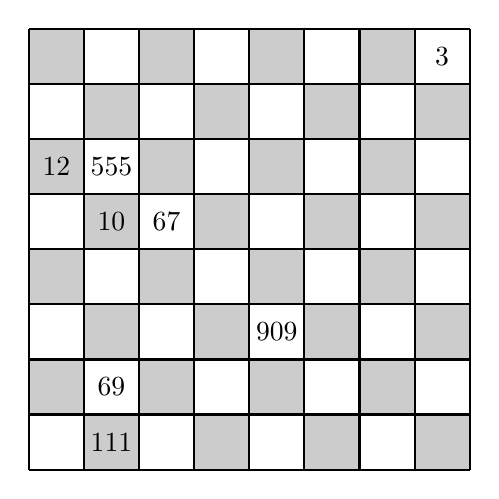
\begin{tikzpicture}[scale=0.7]

            \foreach \x in {0,1,...,7} {
                \foreach \y in {0,1,...,7} {
                    \pgfmathparse{mod(\x+\y,2) ? "black!20" : "white"}
                    \edef\col{\pgfmathresult}
                    \fill[\col] (\x,\y) rectangle (\x+1,\y+1);
                }
            }

            \node at (1.5,0.5) {111}; \node at (1.5,1.5) {69}; \node at (4.5,2.5) {909}; \node at (1.5,4.5) {10};
            \node at (2.5,4.5) {67}; \node at (0.5,5.5) {12}; \node at (1.5,5.5) {555}; \node at (7.5,7.5) {3};

            \draw[thick] (0,0) grid (8,8);
        \end{tikzpicture}
        \vspace{1.5em}
        \caption*{Random values corresponding to each piece and the \textit{en passant} square. The value for black to move is 62319.}
    \end{minipage}
    \caption{Zobrist hash calculation example.}\label{fig:zobristExamplePosition}
\end{figure}

\subsection*{Table entry}

Each entry in the transposition table stores the following information:

\begin{enumerate}
  \item \textit{Zobrist Hash}: The full 64-bit hash of the position. This is used to verify that the entry corresponds to the current position and to detect possible index collisions in the table.
  \item \textit{Evaluation}: The numerical evaluation of the position, as computed by the evaluation function.
  \item \textit{Depth}: The depth at which the evaluation was calculated. A deeper search could potentially yield a more accurate evaluation, so this value helps determine whether a new evaluation should overwrite the existing one.
  \item \textit{Node Type}: Indicates the type of node stored:
  \begin{enumerate}
    \item \textit{EXACT} the evaluation is precise for this position.
    \item \textit{UPPERBOUND} the evaluation is an upper bound, typically resulting from an alpha cutoff.
    \item \textit{LOWERBOUND} the evaluation is a lower bound, typically resulting from a beta cutoff.
    \item \textit{FAILED} entry is empty or with invalid information.
  \end{enumerate}
\end{enumerate}

\subsection*{Collisions}

As discussed earlier, index collisions in the transposition table are handled by verifying the full Zobrist hash stored in the entry. However, it is still theoretically possible for a full hash collision to occur, that is two different positions producing the same hash.

\vspace{1em}

\noindent This scenario is extremely rare. With 64-bit hashes, there are $2^{64}$ possible unique values, which is more than sufficient for practical purposes. In the unlikely event of a true hash collision, it could result in an incorrect evaluation being reused for a different position.

\section{Move generator with magic bitboards and pext instructions}

As previously discussed (see~\cref{sec:moveGenerator}), computing the legal moves for sliding pieces is computationally expensive, as it requires identifying which pieces block their paths within their attack patterns. In this section, we present a technique that enables the precomputation of all possible moves for rooks and bishops, while queen moves can be derived as the union of rook and bishop moves, allowing constant-time O(1) access.

\subsection*{Magic bitboards}

We can create a look up table of all the rook and bishop moves for each square on the board and for each combination of pieces that blocks the path of the slider piece (blockers  bitboard). Basically we need a hash table to store rook and bishop moves indexed by square and bitboard of blockers. The problem is that this table could be very big~\cite{MagicBitboards}.

\vspace{1em}

\noindent Magic bitboards technique used to reduce the size of the look up table. We cut off unnecessary information in the blockers bitboard, excluding the board borders and the squares outside its attack pattern.

\vspace{1em}

\noindent A \textbf{magic number} is a multiplier to the bitboard of blockers with the following properties:

\begin{itemize}[itemsep=1pt]
  \item Preserves relevant blocker information: 
    Only the nearest blockers along a sliding piece's movement direction are important. For example, in~\cref{fig:magics_position}, the pawn on d6 is a relevant blocker because it directly restricts the rook's movement. In contrast, the pawn on d7 is irrelevant, as it lies beyond the first blocker and does not influence the final set of legal moves.

  \item Compresses the blocker bitboard, pushing the important bits near the most significant bit.
  \item The final multiplication must produce a unique index for each possible blocker configuration. The way to ensure the uniqueness is by brute force testing.
\end{itemize}

\noindent We aim to compute the legal moves of the white rook in the given position. In practice, the only pieces that truly block the rook's path are those marked with a red circle.

\vspace{1em}

\begin{figure}[H]
    \centering
    \newchessgame
    \chessboard[
        showmover=false,
        setfen=n1bk3r/3p4/1p1p2p1/8/3R1p2/8/3p4/7n w - - 0 1,
        markstyle=border,
        color=red, markfields={d6,f4,d2},
        color=green, markfields={c4,b4,a4,e4,d5,d3}
    ]
    \caption{Chess position with white rook legal moves in green and blockers in red.}\label{fig:magics_position}
\end{figure}

\subsection*{Magic number generation}

\noindent
Magic numbers are generated through a trial and error process. For each square on the board,random numbers are tested until one produces a unique index for every possible blocker configuration~\cite{MagicBitboards}. Over the years, the chess programming community has discovered better magic numbers. In this project, we use magics sourced from the Chess Programming YouTube channel~\cite{MagicsSource}.


\subsection*{Index calculation}

\noindent First, we mask out all pieces outside the rook's attack pattern or on the board borders, as shown i the image below.

\vspace{1em}

\begin{figure}[H]
    \centering
    \begin{minipage}[c]{0.4\textwidth}
        \centering
        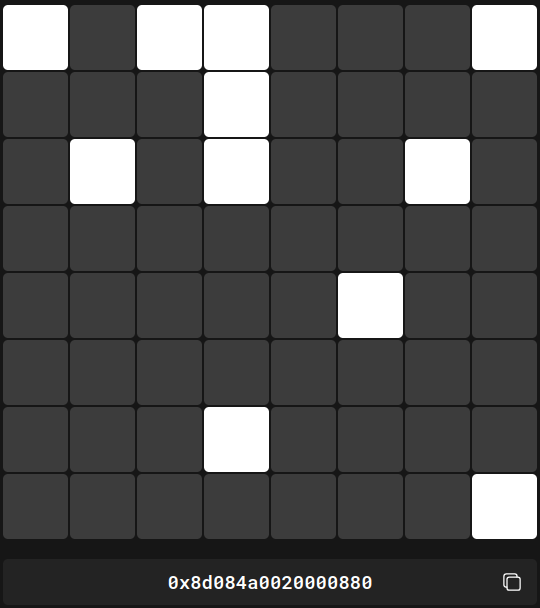
\includegraphics[width=\textwidth]{Imagenes/magics_blockers.png}
        \caption{Original blockers bitboard}
    \end{minipage}
    \hfill
    \begin{minipage}[c]{0.1\textwidth}
        \centering
        \small$\to$
    \end{minipage}
    \hfill
    \begin{minipage}[c]{0.4\textwidth}
        \centering
        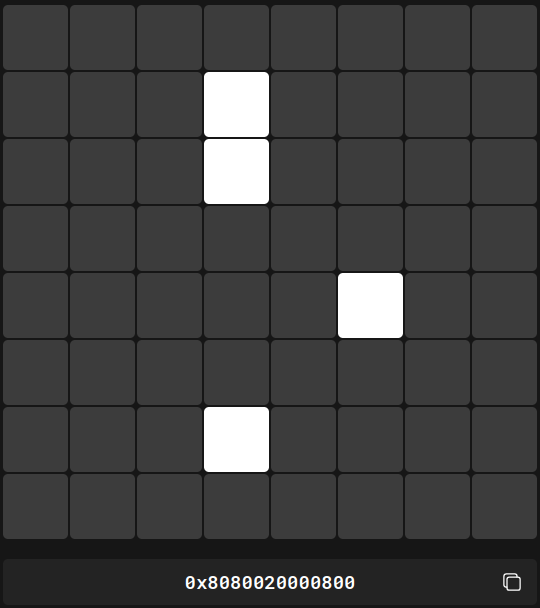
\includegraphics[width=\textwidth]{Imagenes/magics_processed_blockers.png}
        \caption{Masked blockers bitboard}
    \end{minipage}
    \caption*{Pre-processing of the blockers bitboard}\label{fig:magic_preprocessing}
\end{figure}

\noindent The masked blockers bitboard is then multiplied by the magic number. The result retains only the three relevant pawns that obstruct the rook's movement, pushing them toward the most significant bits.

\vspace{1em}

\begin{figure}[H]
    \centering
    \begin{minipage}[c]{0.4\textwidth}
        \centering
        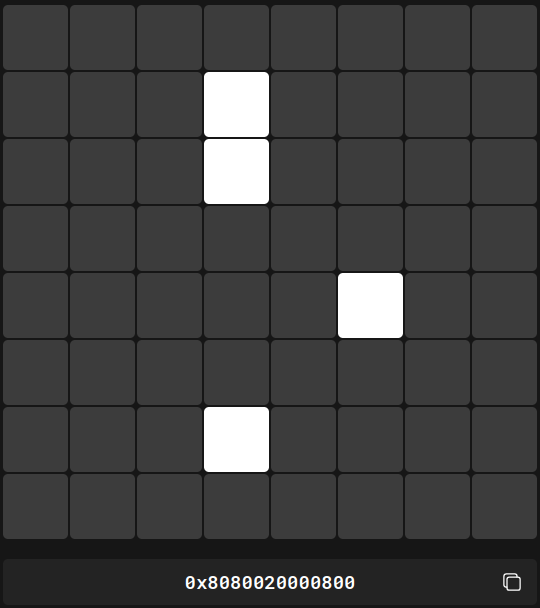
\includegraphics[width=\textwidth]{Imagenes/magics_processed_blockers.png}
        \caption{Masked blockers bitboard}
    \end{minipage}
    \hfill
    \begin{minipage}[c]{0.1\textwidth}
        \centering
        \Huge$\times$ \\[0.5em]
        \small Magic number \\[0.5em]
        \Huge$=$
    \end{minipage}
    \hfill
    \begin{minipage}[c]{0.4\textwidth}
        \centering
        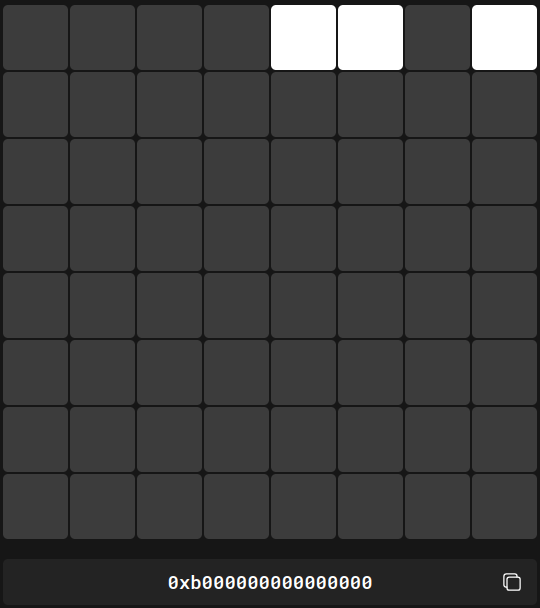
\includegraphics[width=\textwidth]{Imagenes/magics_multiplied_blockers.png}
        \caption{Multiplied blockers bitboard}
    \end{minipage}
    \caption*{Multiplication by magic number to produce an index}\label{fig:magic_multiplication}
\end{figure}

\noindent Next, we compress the index toward the least significant bits by shifting right by \(\,64-\)\texttt{relevant\_squares}. The number of relevant squares varies per board square;~\cref{fig:rook_relevant_squares} shows this for the rook:

\vspace{1em}

\begin{figure}[H]
    \centering
    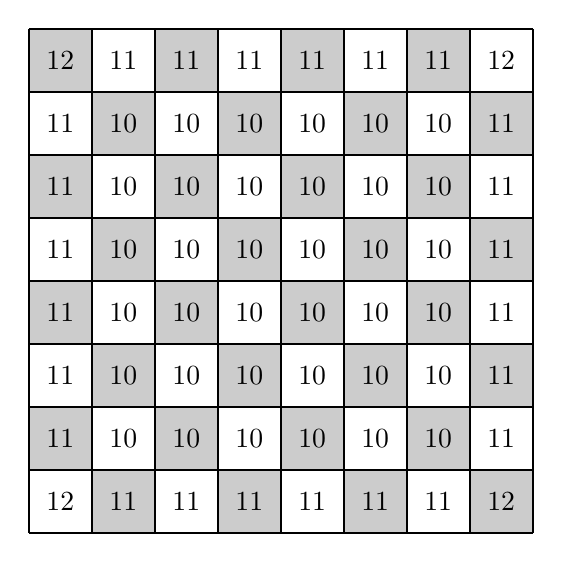
\begin{tikzpicture}[scale=0.8]
        % Draw the chessboard
        \foreach \x in {0,1,...,7} {
            \foreach \y in {0,1,...,7} {
                \pgfmathparse{mod(\x+\y,2) ? "black!20" : "white"}
                \edef\col{\pgfmathresult}
                \fill[\col] (\x,\y) rectangle (\x+1,\y+1);
            }
        }

        % Add the values to the squares
        \node at (0.5,7.5) {12}; \node at (1.5,7.5) {11}; \node at (2.5,7.5) {11}; \node at (3.5,7.5) {11};
        \node at (4.5,7.5) {11}; \node at (5.5,7.5) {11}; \node at (6.5,7.5) {11}; \node at (7.5,7.5) {12};

        \node at (0.5,6.5) {11}; \node at (1.5,6.5) {10}; \node at (2.5,6.5) {10}; \node at (3.5,6.5) {10};
        \node at (4.5,6.5) {10}; \node at (5.5,6.5) {10}; \node at (6.5,6.5) {10}; \node at (7.5,6.5) {11};

        \node at (0.5,5.5) {11}; \node at (1.5,5.5) {10}; \node at (2.5,5.5) {10}; \node at (3.5,5.5) {10};
        \node at (4.5,5.5) {10}; \node at (5.5,5.5) {10}; \node at (6.5,5.5) {10}; \node at (7.5,5.5) {11};

        \node at (0.5,4.5) {11}; \node at (1.5,4.5) {10}; \node at (2.5,4.5) {10}; \node at (3.5,4.5) {10};
        \node at (4.5,4.5) {10}; \node at (5.5,4.5) {10}; \node at (6.5,4.5) {10}; \node at (7.5,4.5) {11};

        \node at (0.5,3.5) {11}; \node at (1.5,3.5) {10}; \node at (2.5,3.5) {10}; \node at (3.5,3.5) {10};
        \node at (4.5,3.5) {10}; \node at (5.5,3.5) {10}; \node at (6.5,3.5) {10}; \node at (7.5,3.5) {11};

        \node at (0.5,2.5) {11}; \node at (1.5,2.5) {10}; \node at (2.5,2.5) {10}; \node at (3.5,2.5) {10};
        \node at (4.5,2.5) {10}; \node at (5.5,2.5) {10}; \node at (6.5,2.5) {10}; \node at (7.5,2.5) {11};

        \node at (0.5,1.5) {11}; \node at (1.5,1.5) {10}; \node at (2.5,1.5) {10}; \node at (3.5,1.5) {10};
        \node at (4.5,1.5) {10}; \node at (5.5,1.5) {10}; \node at (6.5,1.5) {10}; \node at (7.5,1.5) {11};

        \node at (0.5,0.5) {12}; \node at (1.5,0.5) {11}; \node at (2.5,0.5) {11}; \node at (3.5,0.5) {11};
        \node at (4.5,0.5) {11}; \node at (5.5,0.5) {11}; \node at (6.5,0.5) {11}; \node at (7.5,0.5) {12};

        % Draw the grid
        \draw[thick] (0,0) grid (8,8);
    \end{tikzpicture}
    \caption{Relevant squares for rook piece.}\label{fig:rook_relevant_squares}
\end{figure}

\noindent The final index is thus computed as:

\begin{align*}
    \text{index} 
    &= (\text{bitboard\_of\_blockers} \times \text{magic\_number})
       \;\gg\;(64 - \text{relevant\_squares})\,.
\end{align*}

\subsection*{PEXT instruction}

\noindent The PEXT (Parallel Bits Extract) is an instruction available on modern CPUs. They extracts bits from a source operand according to a mask and packs them into the lower bits of the destination operand~\cite{PextInstruction}. It is ideally suited for computing our table index.

\vspace{1em}

\noindent\cref{fig:pext_instruction_example} illustrates how PEXT works: it selects specific bits from register \texttt{r2}, as specified by the mask in \texttt{r3}, and packs the result into the lower bits of the destination register \texttt{r1}.

\vspace{1em}

\begin{figure}[H]
    \centering
    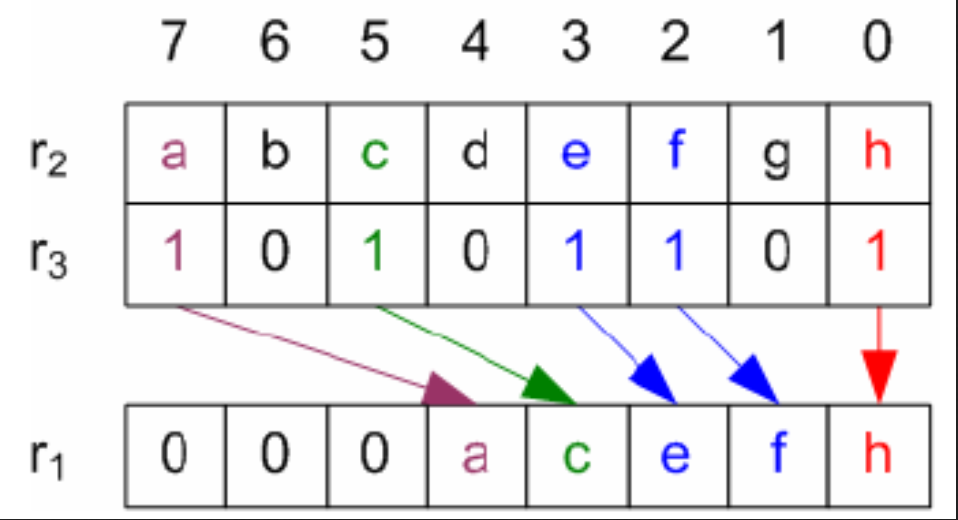
\includegraphics[width=0.5\textwidth]{Imagenes/pext.png}
    \caption{Example of the PEXT instruction.}\label{fig:pext_instruction_example}
\end{figure}

\noindent For our previous example (see~\cref{fig:magics_position}), we only need the full bitboard of blockers and the rook's attack pattern (excluding the borders to reduce space), as illustrated below.

\vspace{1em}

\begin{figure}[H]
    \centering
    \begin{minipage}[c]{0.3\textwidth}
        \centering
        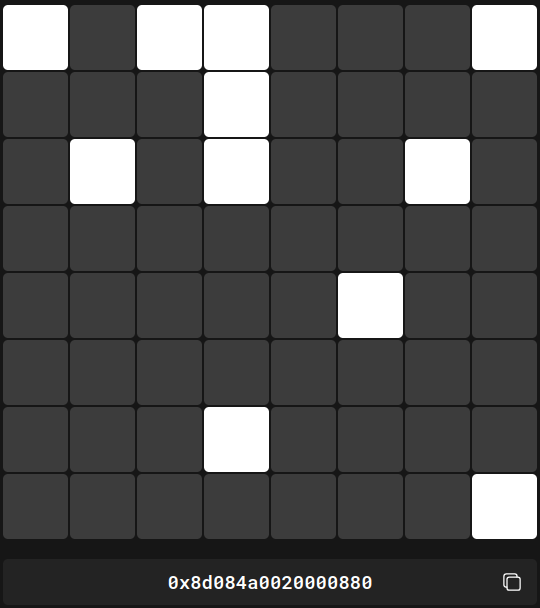
\includegraphics[width=\textwidth]{Imagenes/magics_blockers.png}
        \caption*{Blockers bitboard}
    \end{minipage}
    \hfill
    \begin{minipage}[c]{0.3\textwidth}
        \centering
        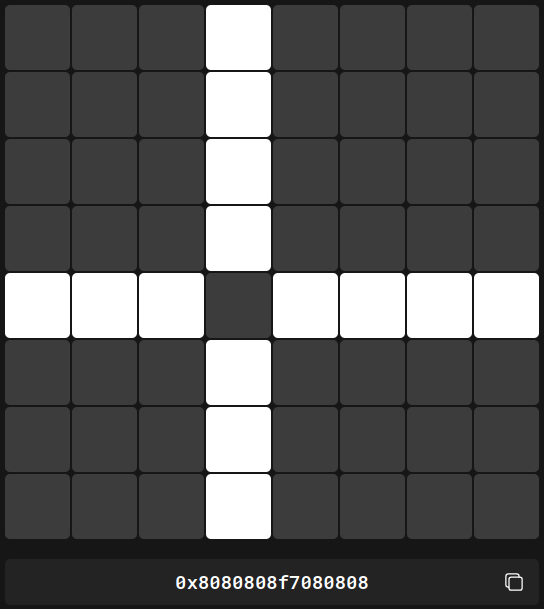
\includegraphics[width=\textwidth]{Imagenes/magics_rook_attacks.png}
        \caption*{Rook attack mask}
    \end{minipage}
    \hfill
    \begin{minipage}[c]{0.05\textwidth}
        \centering
        \Huge\texttt{$\rightarrow$}
    \end{minipage}
    \hfill
    \begin{minipage}[c]{0.3\textwidth}
        \centering
        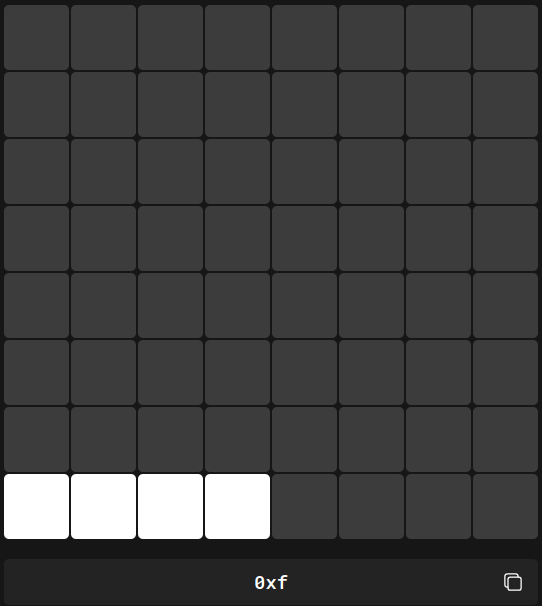
\includegraphics[width=\textwidth]{Imagenes/pext_final_index.png}
        \caption*{Final extracted index}
    \end{minipage}
    \caption*{Index extraction with PEXT example.}\label{fig:pext_bitboards}
\end{figure}

\noindent The final index used to access the lookup table is calculated using the PEXT instruction as follows:
\begin{align*}
    \text{index}
    &= \text{\_pext\_u64}(\text{blockers},\,\texttt{attack\_pattern})\,.
\end{align*}

\subsection*{Conditional implementation}

\noindent To maintain compatibility and performance across different hardware platforms, we provide two implementations for computing the indices:

\begin{itemize}[itemsep=1pt]
  \item If PEXT support is detected at compile time, the engine uses it to compute the index directly.
  \item Otherwise, the engine falls back to the magic bitboards approach using multiplication and bit shifts.
\end{itemize}

\section{Evaluation with king safety and piece mobility}

While material count is the fundamental part for evaluating a chess position, human players also consider strategic and positional factors such as pawn structure, piece activity and king safety. We extend the evaluation function by incorporating additional parameters. These enhancements aim to produce a more accurate assessment of the position.

\subsection*{King shield bonus}

The king is typically safer when protected by friendly pawns in front of it. We assign a bonus in the evaluation score for each allied pawn positioned directly in front of the king. In the following image the white side has one pawn in front of the king, adding 100 bonus points, while black has 3 pawns adding 300 bonus shield points.

\begin{center}
    \newchessgame
    \chessboard[
        showmover=false,
        setfen=r1b2rk1/1ppp1ppp/2n5/p1b1p2n/2B1P2q/2NP1N2/PPP2P2/R1BQ1RK1 b - - 7 15,
        markstyle=border,
        color=green, markfields={f2},
        color=blue, markfields={f7,g7,h7}
    ]
\end{center}

\subsection*{King safety penalty}

To evaluate the safety of the king, we analyze the $3 \times 3$ area surrounding the king, counting how many enemy pieces attack any of those squares. Each type of attacking piece contributes a different \textit{threat weight}:

\begin{itemize}
    \item Queen: 4 points.
    \item Rook: 3 points.
    \item Bishop/Knight: 2 points.
    \item Pawn: 1 point.
\end{itemize}

\par We sum these threat values to compute a \textit{total danger score}. This score is then used as an index into the \textit{precomputed safety table}~\cref{tab:safetyTable}, which returns the corresponding penalty to apply to the evaluation score. This method allows us to smoothly scale the penalty based on the level of threat around the king. The maximum penalty applied is 500 points.

\begin{table}[H]
\centering
\caption{Sample entries from the king safety penalty table.}
\begin{tabular}{|c|c|c|c|c|c|c|c|c|c|c|}
\hline
\textit{Threat Score}     & 0 & 1 & 2 & 3 & 5 & 10 & ... & 20 & ... & 61 \\
\hline
\textit{Penalty} & 0 & 0 & 1 & 2 & 5 & 18 & ... & 68 & ... & 500 \\
\hline
\end{tabular}
\label{tab:safetyTable}
\end{table}

\par In the following image, the black king is under threat from multiple pieces: the queen attacks two squares (8 points), the rook attacks three squares (9 points), a knight attacks one square (2 points), and a pawn attacks one square (1 point). This results in a total threat score of 20, which corresponds to a penalty of 68 points according to the safety table.

\begin{center}
    \newchessgame
    \chessboard[
        showmover=false,
        setfen=7k/5pnp/1p6/p2P4/2Np4/8/8/K1Q4R w - - 0 1,
        markstyle=border,
        color=green, markfields={g8,f8,e8,e7,f7,g7,f6,g6,f5},
        color=red, markfields={h5,h6,h7,e6,e5,g5}
    ]
\end{center}

\subsection*{Piece mobility}

Greater piece mobility is generally indicative of a stronger position. Each piece receives a bonus for every available move to a square that is not attacked by enemy pawns. 

\vspace{1em}

To implement this feature, we first compute a bitboard representing all legal moves available to a given piece. We then apply a mask that removes any squares attacked by enemy pawns. The resulting bitboard contains only safe mobility squares. For example in the following image the queen has twelve legal moves to squares not attacked by enemy pawns, and therefore receives a mobility bonus of 12 points. The safe squares are highlighted in green.

\begin{center}
    \newchessgame
    \chessboard[
        showmover=false,
        setfen=rn2kbnr/pppbpppp/8/3q4/7P/8/PPPP1PP1/RNBQKBNR b KQkq - 0 1,
        markstyle=border,
        color=red, markfields={g5,f3,d3,b3},
        color=green, markfields={d4,d6,e5,f5,h5,c5,b5,a5,c4,e6,c6,e4}
    ]
\end{center}

\newpage
\section{Multithreaded search}

This version of search follows Young Brothers Wait Concept, which is a parallel search algorithm designed to optimize the distribution of work among multiple threads.

\vspace{1em}

\noindent This is particularly effective in alpha-beta pruning, where the search tree is explored selectively. It is divided into two phases: the principal variation move and the wait concept.

\vspace{1em}

\noindent The principal variation is searched sequentially by the main thread, ensuring that the most promising move is evaluated first. If this move turns out to be the best and pruning is applied, the search can directly return the final node evaluation. Otherwise, once the first move has been evaluated, the remaining moves are distributed among multiple threads for parallel evaluation. The wait concept refers to these threads that remain idle until the main thread finishes searching the principal variation.

\vspace{1em}

\noindent In~\cref{fig:pvsplitting}, the gray circle and square nodes are considered part of the principal variation, while the remaining white nodes are processed in parallel by multiple threads.

\begin{figure}
   \centering
   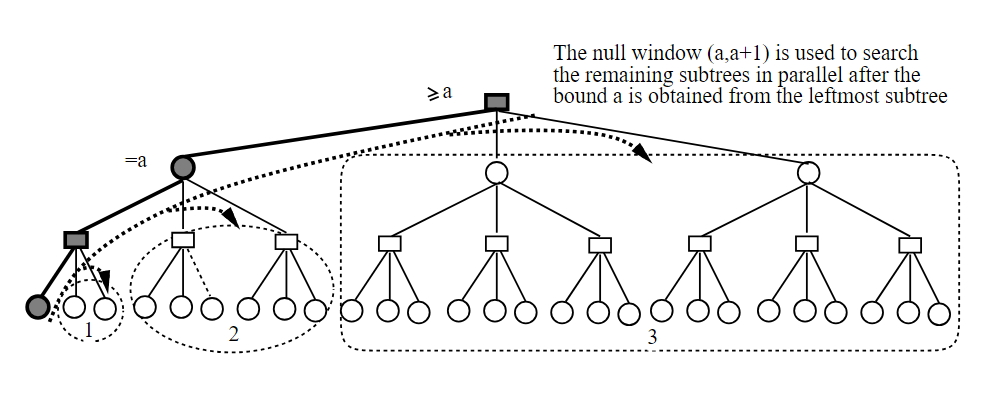
\includegraphics[width=0.9\textwidth]{Imagenes/Bitmap/pvsplitting.png}
   \caption{Principal variation splitting~\cite{PVSplitting}.}\label{fig:pvsplitting}
\end{figure}

\newpage
\section{Late move reductions}

\noindent We experiment with the use of late move reductions, a search optimization technique that selectively reduces the search depth for moves that appear late in the move ordering and are therefore considered less promising~\cite{LateMoveReductions}. The technique is based on the assumption that a strong move ordering heuristic will place the best move in the position earlier in the list. As a result, moves evaluated later can be searched at a reduced depth to save computation time.

\vspace{1em}

\par
In our implementation, a reduction of one ply is applied to non-capturing moves when the side to move is not in check, the remaining search depth is at least three plies, and the move index is beyond a threshold of the 10th move. The reduction condition is formally defined in the following equation:

\begin{equation*}
\text{reduction} = 
\begin{cases}
1, & \text{if } \text{isNotCheck} \wedge \text{depth} \geq 3 \wedge moveIndex \geq 10 \\
0, & \text{otherwise}
\end{cases}
\end{equation*}

\vspace{1em}

\par
If the reduced-depth search returns a score within the alpha-beta window ($\alpha < \text{eval} < \beta$), indicating that the move may be stronger than initially assumed, a full-depth re-search is triggered to ensure it is not mistakenly pruned.


